\chapter{Preliminaries}

\section{Motivation}

Neurological and cognitive conditions such as amyotrophic lateral sclerosis, brain strokes, and spinal injuries can potentially disrupt the communication pathways within the human brain, affecting voluntary muscle control used to communicate with the external environment, such as locked-in syndrome \cite{sisti2022brief, mcfarland2011brain}. To address this, Brain-Computer Interfaces (BCIs) have surged in interest as they are computer-based systems that capture and analyze brain signals, translating them into commands \cite{khan2020review, ramadan2015basics}. 

Motor Imagery (MI), an extensively studied paradigm within BCI research, particularly holds promise in the recovery of motor functionality \cite{bonci2021introductory}. Clinical integrations of MI-BCIs with skilled therapists have proven beneficial in aiding the sensory or motor rehabilitation process, facilitating better environmental interaction for people with neurological disorders \cite{sitaram2017closed, hochberg2012reach,lebedev2006brain}. Beyond clinical applications, MI-BCI systems have seen increased use in non-clinical settings such as virtual reality, gaming, and skill acquisition among healthy subjects \cite{cattan2018recommendations}. Iconic video games such as Pong and Pacman can be played using MI, and studies on healthy subjects show promise in facilitating skills acquisition across various disciplines \cite{ahn2014review, ganin2013p300, johnson2018combined, perdikis2018cybathlon}. 

Nowadays, interest in BCI systems has grown to such a point that before the COVID-19 pandemic, there were more than 150 BCI-based companies distributed in sectors such as automotive, aerospace, medical technology, rehabilitation, robotics, entertainment, marketing, and technology. Besides, the European Commission leads a program called 'The Future of Brain/Neural Computer Interaction: Horizon 2020' to establish a worldwide coordination effort by funding and supporting actions as well as defining a roadmap for future research, taking into account market needs until 2025~\cite{brunner2015bnci}. For instance, the BCI technology market, valued at USD 228.1 million in 2022, is expected to witness substantial growth, with an estimated value of USD 460.1 million by 2029, according to a recent market report \footnote{\url{https://www.marketreportsworld.com/enquiry/request-sample/23789843}}. From a demographic perspective, the value of BCI technology in global socioeconomic development is acknowledged. However, the method for studying this technology varies depending on the specific context of each country, with the USA and China leading in the number of scientific publications, followed by Germany, Japan, and India~\cite{maiseli2023brain}. In this sense, BCI technology development must adhere to the fundamental ideals of humanity, including convenience, ease-of-use, privacy, security, and safety~\cite{willett2021high, matemba2020technology}. 

Neuroimaging techniques are crucial for acquiring brain signals in MI-BCI systems, each playing distinct roles in understanding brain functionality. For instance, Electroencephalography (EEG) and Magnetoencephalography (MEG) capture electrical activity and magnetic fields in the brain, respectively \cite{altaheri2023deep,philip2022non}. Functional Magnetic Resonance Imaging (fMRI) detects changes in blood flow, indicating brain activity \cite{sorger2020real}. Computed Tomography (CT) and Magnetic Resonance Imaging (MRI) provide detailed structural images of the brain, useful in pathology identification \cite{singh2021comprehensive}. Positron Emission Tomography (PET) and Single-Photon Emission Computed Tomography (SPECT) map functional processes in the brain using radioactive substances, highlighting areas with high metabolic activity \cite{veena2020review}. These neuroimaging techniques are summarized in \cref{table:neuroimaging}.

\begin{table}[h]
\centering
\caption{Common neuroimaging techniques principle and working mechanism description}\label{table:neuroimaging}
\scalebox{0.9}{
\begin{tabular}{|l|l|l|}
\hline
\textbf{Technique} & \textbf{Principle} & \textbf{Working Mechanism} \\
\hline
EEG & Records electrical activity & Electrodes on scalp capture voltage fluctuations \\
\hline
MEG & Measures magnetic fields & Superconducting sensors detect magnetic fields \\
\hline
fMRI & Measures blood oxygenation & Detects blood flow changes associated with neural activity \\
\hline
CT & Uses X-rays & X-rays create cross-sectional images \\
\hline
MRI & Uses strong magnetic fields & Protons emit signals for detailed structural images  \\
\hline
PET & Measures emitted gamma rays & Radioactive tracers indicate areas with high metabolic activity\\
\hline
SPECT & Measures emitted gamma rays & Tracers indicate areas with high blood flow\\
\hline
\end{tabular}
}
\end{table}

\cref{fig:neuroimagig} shows the spatial and temporal resolutions and relative cost comparison among the previously mentioned techniques. The color gradient in the figure represents the relative cost of each neuroimaging technique, with green indicating more affordable options and red signifying higher expenses. EEG and MEG are notable for their high temporal resolution, capturing rapid changes in brain activity with millisecond precision \cite{shao2020eeg}. In contrast, fMRI provides excellent spatial resolution, offering detailed insights into brain structures and activity \cite{yuan2021bci}. However, fMRI has a slower temporal resolution than EEG and MEG, making it less suitable for capturing rapid neural dynamics \cite{li2021review}. CT scans, which use X-rays to create cross-sectional images, and MRIs, which use powerful magnetic fields and radio waves, thus avoiding ionizing radiation, both provide detailed anatomical information about the brain's morphology \cite{zhuang2020state}. PET and SPECT focus on functional imaging by detecting radioactive tracers and can reveal metabolic and neurotransmitter activity, but their temporal resolution is relatively lower than EEG and MEG \cite{ramadan2017brain}. While spatial and temporal resolutions are critical factors in selecting the appropriate neuroimaging method, the cost aspect is equally important for decision-making in various research and clinical contexts \cite{rashid2020current}."

\begin{figure}[h!]
    \centering
    \resizebox{0.8\linewidth}{!}{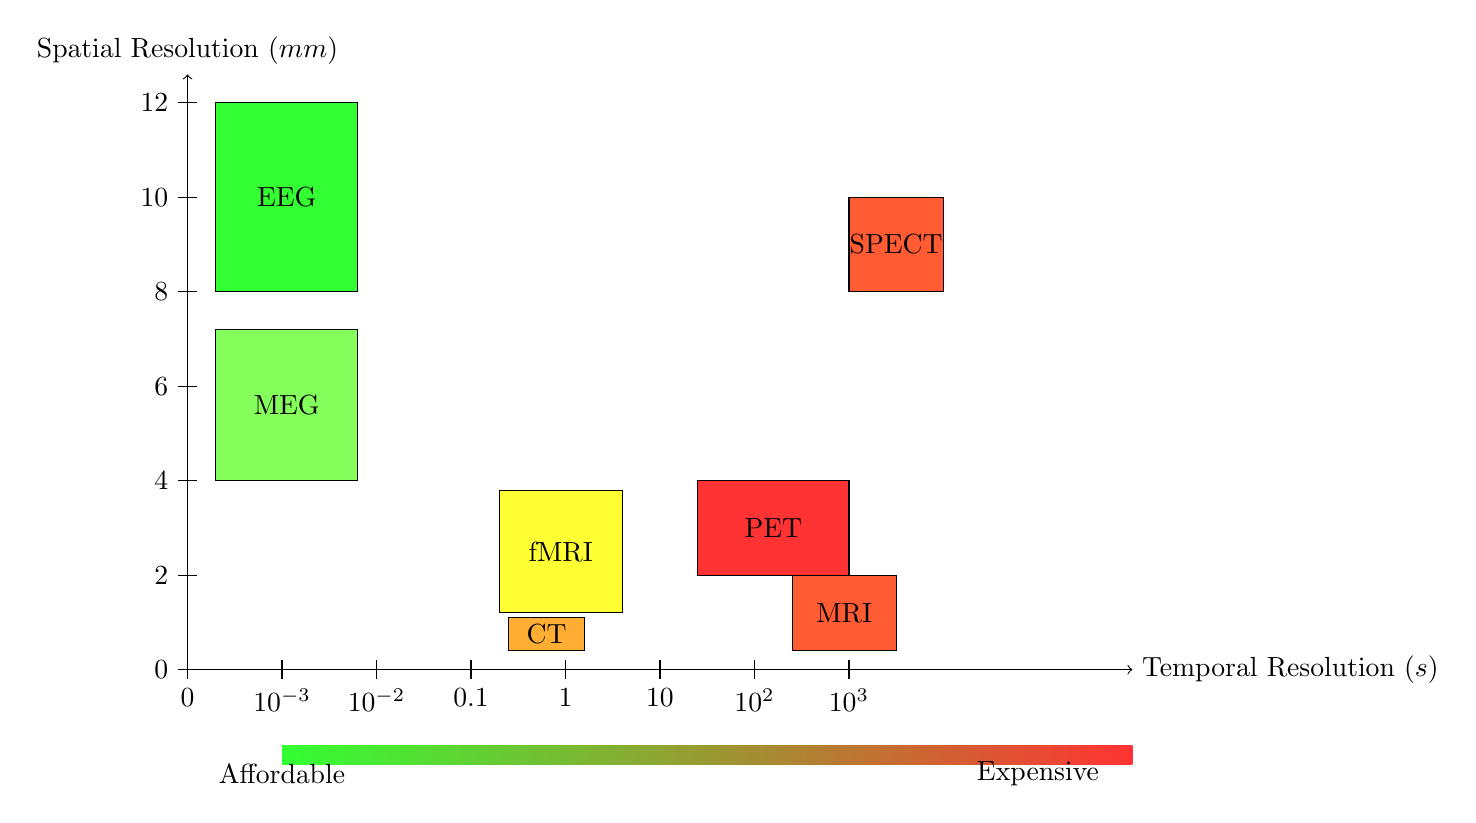
\begin{tikzpicture}[scale=1.2]

% Draw axes
% EEG 0.2
% MEG 0.4
% fMRI 0.8
% CT 0.6
% MRI 0.7
% PET 0.9
% SPECT 0.8

\definecolor{eegcolor}{HTML}{00FF00}
\definecolor{megcolor}{HTML}{66FF33}
\definecolor{fmricolor}{HTML}{FFFF00}
\definecolor{ctcolor}{HTML}{FF9900}
\definecolor{mricolor}{HTML}{FF3300}
\definecolor{petcolor}{HTML}{FF0000}
\definecolor{spectcolor}{HTML}{FF3300}
% X-axis labels
\draw[->] (0,0) -- (10,0) node[right] {Temporal Resolution $(s)$};
\draw (0,0.1) -- (0,-0.1) node[below] {$0$};
\draw (1,0.1) -- (1,-0.1) node[below] {$10^{-3}$};
\draw (2,0.1) -- (2,-0.1) node[below] {$10^{-2}$};
\draw (3,0.1) -- (3,-0.1) node[below] {$0.1$};
\draw (4,0.1) -- (4,-0.1) node[below] {$1$};
\draw (5,0.1) -- (5,-0.1) node[below] {$10$};
\draw (6,0.1) -- (6,-0.1) node[below] {$10^2$};
\draw (7,0.1) -- (7,-0.1) node[below] {$10^3$};

% Y-axis labels
\draw[->] (0,0) -- (0,6.3) node[above] {Spatial Resolution $(mm)$};
\draw (0.1,0) -- (-0.1,0) node[left] {$0$};
\draw (0.1,1) -- (-0.1,1) node[left] {$2$};
\draw (0.1,2) -- (-0.1,2) node[left] {$4$};
\draw (0.1,3) -- (-0.1,3) node[left] {$6$};
\draw (0.1,4) -- (-0.1,4) node[left] {$8$};
\draw (0.1,5) -- (-0.1,5) node[left] {$10$};
\draw (0.1,6) -- (-0.1,6) node[left] {$12$};

\fill[left color=eegcolor!80, right color=petcolor!80] (1,-1) rectangle ++(9,0.2);

\draw (9,-1.1) node[align=center] {Expensive};
\draw (1,-1.1) node[align=center] {Affordable};

% EEG (x,y)
\draw[fill=eegcolor!80] (0.3,4) rectangle (1.8,6) node[pos=.5] {EEG};

% MEG
\draw[fill=megcolor!80] (0.3,2) rectangle (1.8,3.6) node[pos=.5] {MEG};

% fMRI
\draw[fill=fmricolor!80] (3.3,0.6) rectangle (4.6,1.9) node[pos=.5] {fMRI};

% CT
\draw[fill=ctcolor!80] (3.4,0.2) rectangle (4.2,0.55) node[pos=.5] {CT};

% MRI
\draw[fill=mricolor!80] (6.4,0.2) rectangle (7.5,1) node[pos=.5] {MRI};

% PET
\draw[fill=petcolor!80] (5.4,1) rectangle (7,2) node[pos=.5] {PET};

% SPECT
\draw[fill=spectcolor!80] (7,4) rectangle (8,5) node[pos=.5] {SPECT};

\end{tikzpicture}}
    \caption{Comparison of neuroimaging techniques: spatial and temporal resolutions, and relative costs}\label{fig:neuroimagig}
\end{figure}

In particular, MI involves fast-evolving cognitive processes that require superior temporal resolution \cite{varbu2022past}. Therefore, EEG and MEG offer valuable options for capturing short-living events and temporal patterns of neural activity, allowing researchers to observe and analyze brain activity with remarkable temporal precision \cite{alsharif2020neuromarketing}. In addition, due to portability and cost-effectiveness, EEG is the neuroimaging technique most extensively studied by researchers and budget-constrained institutions focusing on MI-BCI applications \cite{janapati2023advances, hosseini2020review, shao2020eeg, khan2020review, lopez2020beyond, ramadan2017brain, fogelson2013functional}. A typical EEG-based MI-BCI system uses a processor unit and an EEG headset equipped with $N_c$ electrodes (channels), varying from $1$ to $256$ \cite{grigorev2021bci, rashid2020current}. These electrodes, attached with an elastic cap, make direct contact with the scalp, recording electrical variations that encode brain activities \cite{varbu2022past}. In addition, some setups may include a monitor for instructing the individual to execute a specific MI task \cite{gu2021eeg}. A visual representation of the setup can be found in \cref{fig:eegsetup}.

\begin{figure}[!ht]
		\centering
		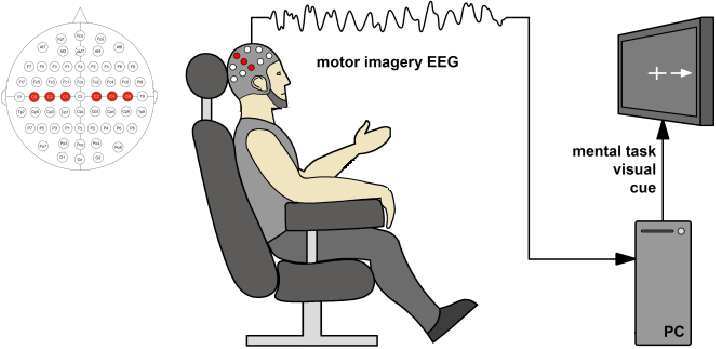
\includegraphics{Figures/preliminaries/EEG-setup.png}
		\caption{Experimental setup for MI-based BCIs. \textbf{{Source}
				:} {Adapted from} \cite{grigorev2021bci}}
		\label{fig:eegsetup}
\end{figure}

Electrical variations recorded by EEG channels are the combination of multiple rhythms that can be used to describe spatially and temporally dynamic patterns of cognitive states within an individual \cite{li2019brain}. The specific neural rhythms that occur in the brain's sensorimotor cortex, an area of the brain involved in planning, controlling, and executing motor functions \cite{leeuwis2021functional}, are known as Sensorimotor Rhythms (SMRs) \cite{altaheri2023deep}. SMRs depend upon individuals and manifest as frequency, shape, and amplitude changes in electrical activity \cite{barios2019synchronization}. In general, most of the cognitive processes implicate six frequency bands: delta [0.5-4]$Hz$, theta [4-8]$Hz$, alpha [8-13]$Hz$, beta [13-30]$Hz$, lower gamma [30-80]$Hz$, and upper gamma [80-150]$Hz$ \cite{khademi2023review, rashid2020current}. Specifically, motor execution and motor imagery actions implicate a frequency range between approximately [4-40] $Hz$ \cite{cattai2021phase}. \cref{tab:freq_bands} describe the most common band types of brain signals according to their frequency ranges.

\begin{table}[h]
    \centering
    \caption{Brain signals classification by frequency range with description}
    \label{tab:freq_bands}
    \begin{tabular}{p{0.15\linewidth}p{0.15\linewidth}p{0.6\linewidth}}
    \hline
      Brain signal  & Frequency range & Description\\
    \hline
      Delta ($\delta$)   & 0.5 to 4 $Hz$ & Slowest brain wave with the highest amplitude, dominant during deep sleep\\
      Theta ($\theta$)  & 4 to 8 $Hz$ & Dominant during deep relaxation and dreaming in light sleep. While normal in children, can be abnormal in awake adults \\
      Alpha ($\alpha$) & 8 to 13 $Hz$ & Dominant in wakeful but relaxed states with closed eyes. \changes{Seen in all ages and can indicate white matter health.}  \\
      Beta ($\beta$) & 13 to 30 $Hz$ & Dominant when alert, concentrated, attentive, and calculating. Typically associated with problem-solving, task engagement, and decision-making  \\
      Lower Gamma ($\gamma_l$)   & 30 to 80 $Hz$ & Active during high-level cognitive tasks \\
      Upper Gamma ($\gamma_u$)   & 80 to 150 $Hz$ & Associated with perception, learning, and language processing \\
      \hline
    \end{tabular}
\end{table}

One of the most important phenomena associated with SMRs is the increase and decrease of oscillatory activity in a particular frequency band during MI tasks, referred to as Event-Related Synchronization (ERS) and Event-Related Desynchronization (ERD) \cite{belwafi2020effective}. ERS and ERD serve as a unique feature of the specific motor action an individual is imagining or executing \cite{zapala2020effects}. This is why several methodologies leverage this critical concept for decoding EEG signals into SMR patterns, aiding in discrimination between MI tasks in EEG-based BCI systems \cite{brusini2021systematic}. 

In general, decoding EEG signals is intricate due to the high sampling rate and number of electrodes, leading to a huge number of data points \cite{singh2021comprehensive}. Therefore, to achieve decent discriminatory capabilities, it is mandatory to perform feature extraction strategies, ensuring a small number of relevant features \cite{ai2019feature}. Feature extraction for MI-BCI systems can be classified into single- or multi-channel approaches.

Single channel perspective relies on the concept of SMRs, and thus, its ultimate goal is to capture oscillatory modulations on specific EEG channels. Time domain strategies collect different temporal information related to a specific MI task, constructing the feature set for a single trial. For instance, statistical features like mean, root mean square, power of the signal, standard deviation variance, skewness, and kurtosis were widely used for MI classification \cite{samuel2017towards, hamedi2014neural}. Other strategies include Hjorth features like activity, mobility, and complexity that indicate the signal power, mean frequency, and change in frequency, respectively \cite{yilmaz2018quasi}. \changes{Simpler strategies like Peak-valley representations, which extract local maximum and local minimum points within a defined timestamp, can also be used to predict MI tasks} \cite{batres2016quaternion}. On the frequency domain side, strategies try to condensate cognitive states within specific frequency bands like in band-power features, that calculates the spectral power in delta, theta, alpha, and beta bands \cite{luo2020motor}; fast Fourier transform, which decomposes EEG signals into its frequency components \cite{rashkov2019natural}; Power Spectral Density (PSD), measuring how the signal power is distributed over frequency \cite{oikonomou2017comparison}. Welch's periodogram, Lomb-Scargle peridiogram, and spectral entropy are methods for extracting or quantifying the PSD of a signal \cite{roy2022comparative, sarraf2017eeg, li2015feature}.

Even though single-channel features can provide useful insights for distinguishing between trials from different MI tasks, it has been shown that oscillatory modulations are not necessarily confined to the sensorimotor cortex \cite{singh2021comprehensive}. Furthermore, the execution or imagination of simple motor tasks activates multiple brain areas that communicate with each other, demonstrating functional integration \cite{ladda2021using}, as opposed to isolated activation of specialized brain regions, known as functional segregation \cite{chiarion2023connectivity}. In brief, by focusing only on single channels, these features may oversimplify the overall phenomenon as they overlook interactions with other regions. Therefore, it is advised to leverage multi-channel feature extraction approaches to provide a more accurate decoding of MI tasks from EEG \cite{leeuwis2021functional}. Among these approaches, the Common Spatial Patterns (CSP) method has been significant in MI-BCI \cite{yang2021multi}. CSP allows the extraction of highly discriminative features by maximizing the separability of SMR features, identifying spatial filters that increase the variance of relevant patterns within one MI process while diminishing the variance of unrelated ones \cite{gaur2021sliding}.

In addition to CSP strategies, Brain Connectivities (BC), which have been used to describe interactions within and between brain regions \cite{ismail2020graph}, can be linked to SMR synchronization mechanisms within EEG recordings \cite{maksimenko2017macroscopic, chiarion2023connectivity}. Key factors of BC include going beyond isolated EEG signals and giving a comprehensive graph visualization that enables researchers to understand brain dynamics between different cognitive states \cite{collazos2023posthoc, grana2023review, tafreshi2019functional, van2014functional, sakkalis2011review}. These factors assist in diagnosing conditions, monitoring progress, and tailoring treatment strategies by tracking how patterns evolve during recovery, therapy, or disease progression \cite{yen2023exploring, lim2021post}. 


\begin{figure}[h]
     \centering
    \begin{subfigure}[b]{.3\linewidth}
        \centering
        \resizebox{1\linewidth}{!}{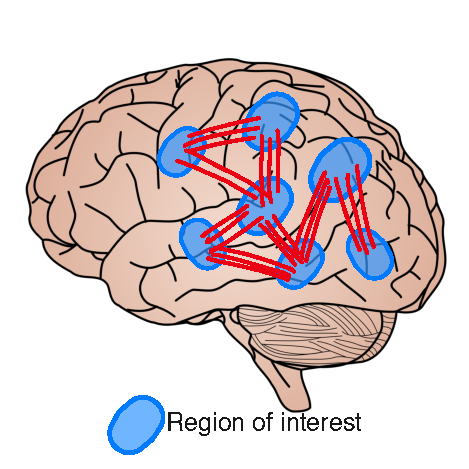
\includegraphics{Figures/preliminaries/SC.pdf}}
        \caption{Structural connectivity\label{fig:SC}}
    \end{subfigure}
    ~
    \begin{subfigure}[b]{.3\linewidth}
        \centering 	\resizebox{1\linewidth}{!}{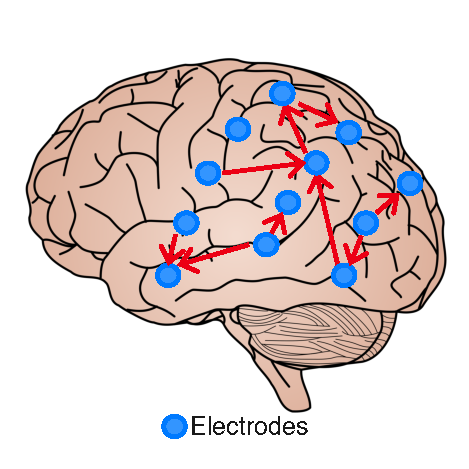
\includegraphics{Figures/preliminaries/EC.pdf}}	
        \caption{Effective connectivity\label{fig:EC}}
    \end{subfigure}
    ~
    \begin{subfigure}[b]{.3\linewidth}
        \centering
        \resizebox{1\linewidth}{!}{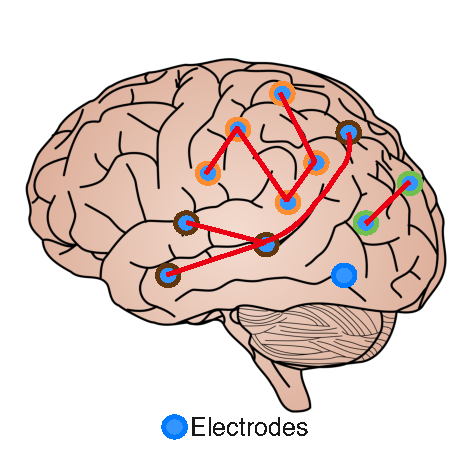
\includegraphics{Figures/preliminaries/FC.pdf}}	
        \caption{Functional connectivity\label{fig:FC}}
    \end{subfigure}
    \caption{Three types of brain connectivities: structural connectivity, effective connectivity, and functional connectivity. Blue circles and blobs represent EEG electrodes and regions of interest, respectively. Circles with different colors represent electrodes with statistical dependencies \label{fig:FC_EC_SC}}
\end{figure}

In general, BC estimates non-directed or directed connections between brain regions and can be divided into three types as depicted in \cref{fig:FC_EC_SC}: Structural/anatomical Connectivity (SC), Effective Connectivity (EC), and Functional Connectivity (FC) \cite{leeuwis2021functional, friston2002functional}. SC, as shown in \cref{fig:SC} focuses on physical connections between different anatomical brain regions, cannot be directly estimated using merely EEG signals and fails to capture short-living events during MI tasks because it is context-independent \cite{thiebaut2020brain, yeh2021mapping}. EC and FC, commonly estimated directly from EEG measures, are suitable for EEG-based MI-BCI systems because they can decode fast-evolving cognitive states \cite{cao2022brain}. According to \cite{friston2013analysing}, EC is always directed and aims to determine how one EEG signal influences another by using parametric models of causal influences as shown in \cref{fig:EC}, while FC can describe directed or non-directed connectives usually via statistical correlation or covariance between EEG signals as shown in \cref{fig:FC}. On one hand, EC requires a deep understanding of the cognitive process to select the most suitable causal model and also demands high computational resources \cite{chiarion2023connectivity, lee2020predicting}. On the other hand, the simplicity of FC, its low computational demands, and the absence of a need for rigid prior assumptions make it particularly well-suited for MI-BCI applications \cite{he2019electrophysiological, hamedi2016electroencephalographic, sakkalis2011review, friston2011functional}.

The Digital Signal Processing and Control Group (DSP\&CG) of Universidad Nacional de Colombia has been working on bio-signal data analysis to propose and develop machine learning methodologies related to automatic systems for the assisted diagnosis of mental conditions \cite{cardenas2017enhanced}, automated analysis of human activity recognition \cite{pulgarin2017relevant}, video analysis based on Multi-Kernel representation \cite{molina2015video}, and biomedical data analysis \cite{hurtado2016identification}. More recently, DSP\&CG works have been focused on extracting relevant patterns from EEG to recognize learning tasks, mainly under the MI paradigm. The used methodologies address dynamic modeling for estimating the spatial relevance of everyday neural activity across subjects \cite{velasquez2020dynamic}, estimation of ERD/S using information theory learning measures \cite{velasquez2020entropy}, enhancement of feature representation based on kernel functional connectivity \cite{garcia2021single}, improving both MI classification and interpretation using convolutional neural networks \cite{collazos2020cnn}. Lastly, BCI performance predictors from deep learning architectures \cite{caicedo2021deep}. Additionally, within \textcolor{black}{the group a variety of research projects are developed}, supported by COLCIENCIAS/MINCIENCIAS, Dirección Nacional de Investigaciones de Manizales (DIMA), and Vicerrectoría de Investigaciones de la Universdiad Nacional de Colombia, such as:

\begin{itemize}
    \item Prototipo de interfaz cerebro-computador de bajo costo para la dectección de patrones relevantes de actividad eléctrica cerebral relacionados con TDAH.
    \item Prototipo de interfaz cerebro-computador multimodal para la dectección de patrones relevantes relacionados con transtornos de impulsividad.
\end{itemize}

From local and general perspectives, integrating MI-BCIs into automatic and semi-automatic rehabilitation systems can provide crucial support for individuals with neurological disorders, aiding in diagnosing conditions, monitoring progress, and tailoring treatment plans. In addition, MI-BCI systems have expanded beyond clinical settings to various applications for healthy subjects, including virtual reality environments, video gaming, and skill acquisition paradigms. EEG's high temporal resolution and affordability make it the most used in MI-BCI clinical and research investigations. Among different feature extraction approaches, multi-channel techniques offer better insights into the actual cognitive state. Specifically, brain connectivity is extensively used in EEG-based MI-BCI systems because it can distinguish between MI tasks; particularly, functional connectivity presents the most suitable strategy for such applications due to their interpretability, low computational demands, and the absence of a need for rigid prior assumptions. The most common issues associated with functional connectivity in EEG-based MI-BCI systems are described in detail in \cref{sec:problem_statement}.